\documentclass[../main.tex]{subfiles}
\begin{document}
\setchapterstyle{kao}
\setchapterpreamble[u]{\margintoc}
\chapter[Matrix Exponential and Logarithm]{Matrix Exponential and Logarithm\footnotemark[0]}
\labch{Matrix-Exponential-and-Logarithm}
%INIZIO LEZIONE 29/04
The matrix exponential and logarithm will be our main tool to make explicit computations, the difference is that the exponential is always well-defined, while the logarithm is not.
\paragraph{Ref:} Hall \cite{Hall2015}, Chapter 2.
\section{Definition \& continuity}
\begin{definition}[Matrix exponential]\index{Matrix exponential}
For $A\in\textrm{Mat}(n,\mathbb{K})\cong \textrm{End}(\mathbb{K}^n)$ for $\mathbb{K}\in \Bqty{\mathbb{R},\mathbb{C}}$, we define the exponential of $A$ as\marginnote[-4mm]{To define a limit we need a topology and the most convenient way to introduce a topology is to introduce a norm.}
\begin{equation}\labeq{def-matrix-exp}
\star \quad \Big|\Big| \qquad e^A=\sum_{m=0}^{+\infty}\frac{1}{m!}A^m=\lim_{N\to+\infty}\sum_{m=0}^N\frac{1}{m!}A^m
\end{equation}
Equip $\textrm{Mat}(n,\mathbb{K})$ with a norm $\norm{\dots}$ satisfying:
\renewcommand{\labelenumi}{\Roman{enumi})}
\begin{enumerate}
    \item $\norm{A+B}\leq \norm{A}+\norm{B}$;
    \item $\norm{AB}\leq\norm{A}\norm{B}$ (if equality even better!);
    \item $\left(\textrm{Mat}(n,\mathbb{K}),\norm{\dots}\right)$ is a \textbf{complete} normed space.
\end{enumerate}
\end{definition}
\begin{marginfigure}[-30mm]
	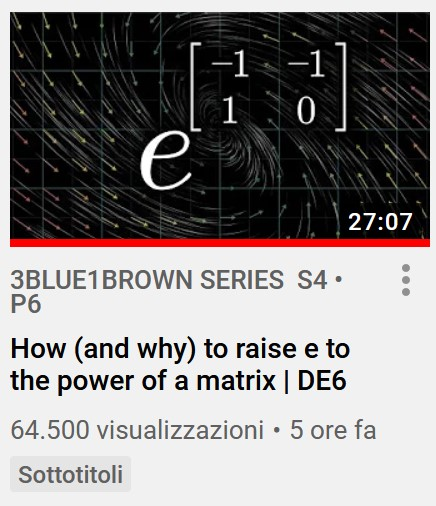
\includegraphics[width=1\linewidth]{images/3blue.jpg}
	\caption[3Blue1Brown video]{Se il lettore volesse avere una spiegazione visiva del significato di esponenziale di una matrice, consigliamo \href{https://www.youtube.com/watch?v=O85OWBJ2ayo}{questo video} di 3Blue1Brown.}
	\labfig{3blue}
\end{marginfigure}
As mathematicians we should ask ourselves if it exists such a norm which satisfies all the three properties, and the answer is that there are infinitely many.
\begin{example}
Hilbert–Schmidt norm
\[
\norm{X}_{\textrm{HS}}=\sum_{i,j=1}^n \abs{X_{ij}}^2=\left(\tr(X^\ast X)\right)^{1/2}
\]
In the last passage we have rewritten it in an intrinsic way (it can be checked that is possible).\marginnote[-2mm]{Intrinsic means without introducing a basis}
\end{example}
The professor's favourite choice is:
\begin{example}Operator norm
\[
\norm{X}=\sup_{v\neq 0}\frac{\norm{Xv}}{\norm{v}}=\sup_{\norm{v}=1}\norm{Xv} \qquad v\in\mathbb{K}^n
\]
where $v$ is intended as a vector in the linear space.
\end{example}
The reason of his preference is the fact that this extends to infinite dimensional Banach spaces, while the firs one does not. But for matrices both are good and equivalent because we are in a finite dimensional linear space. Now we want to prove that \refeq{def-matrix-exp} is convergent.
\begin{theorem}
\labthm{expA}
The series (\ref{eq:def-matrix-exp}) is $\norm{\dots}$-convergent for every\\ $A\in\textrm{Mat}(n,\mathbb{K})$. Moreover, the map $A\mapsto e^A$ is \textbf{continuous} on $\textrm{Mat}(n,\mathbb{C})$. \marginnote{Therefore is continuous globally. We will see that not the same can be said about the logarithm. The latter will be locally defined and locally continuous.}
\end{theorem}
\begin{proof}
We use the fact that as $\left(\textrm{Mat}(n,\mathbb{K}),\norm{\dots}\right)$ is a \underline{\textbf{complete}} normed space, every Chauchy sequence is convergent. Consider the truncated sum:
\[
S_N=\sum_{m=0}^N\frac{1}{m!}A^m \qquad (N\in\mathbb{N})
\]
So we want to prove that the family of all of them $\Bqty{S_N}_{N\in\mathbb{N}}$ is \textbf{Cauchy sequence}: $\forall \ \varepsilon > 0 \ \exists \ N_\ast: \ \forall\;M,N>N_\ast$\marginnote{The only difference with respect to what we did in \textit{Analysis 1} is that now the elements of the sequence are matrices, so we have to take the norm of matrices}
\[
\norm{S_M-S_N}<\varepsilon
\]
Fix $\varepsilon>0$, w.l.o.g.\sidenote{w.l.o.g. = without loss of generality} we can say that $M>N$ (always true up to relabelling). We compute:
\WithArrowsOptions{displaystyle}
\[
\begin{WithArrows}
S_M-S_N&=\sum_{{\color{red}m=N+1}}^{{\color{red}M}}\frac{1}{m!}A^m\Arrow{evaluate the norm}\\
\norm{S_M-S_N}&=\norm{\sum_{{\color{red}m=N+1}}^{{\color{red}M}}\frac{1}{m!}A^m}\leq \Arrow{By triangular inequality I)\\and property II)}\\
&\leq \sum_{m}\frac{1}{m!}\norm{A}^m{\color{red}\overset{?}{<}\varepsilon \quad \textrm{for $M,N$ sufficiently large}}  
\end{WithArrows}
\]
Yes, because $\sum_m^N\frac{1}{m!}\norm{A}^m\xrightarrow[N\to+\infty]{}e^{\norm{A}}\in\mathbb{R}$, so as it is convergent the truncated one, here $\Bqty{S_n}$ is a Cauchy sequence. So we can make it smaller than $\varepsilon$ for $M,N$ sufficiently large, and hence the limit (the \refeq{def-matrix-exp}) exists.

\paragraph{\underline{Continuity}.} As operations in $\textrm{Mat}(n,\mathbb{K})$ are continuous, it turns out that the following map:\marginnote{If the operations are continuos, than the polynomials are continuos.}
\[
A\mapsto \sum_{m=0}^N\frac{1}{m!}A^m=S_N(A)
\]
is \textbf{continuous.} Now we take the norm limit, which tells us that we have a uniform convergence on every compact. \marginnote{Take the ball of radius $R$ in the space of matrices, as we have norm convergence and therefore uniform convergence on every ball of every radius we want. But the exponential is the uniform limit of this polynomial and then it will be continuous on every sphere (and since the radius is arbitrary it is continuous everywhere).} So the polynomial, which is the truncated sum, is continuous in $A$, then, as $S_N(A)\to e^A$ in norm, there is \textbf{uniform convergence on every}\marginnote[-17mm]{One uses the ball if do not want to say \textit{compact set}} $\overline{\mathbb{B}}_R(0)\subseteq \textrm{Mat}(n,\mathbb{K})$. The uniform limit of the continuous functions $S_N(\;\cdot\;)$ is \textbf{continuous}, hence $\overline{\mathbb{B}}_R(0)\ni A \mapsto e^A$ is continuous. As $R$ is arbitrary, we concluded.
\end{proof}
\begin{kaobox}[frametitle=Remark]
Exactly the same proof, with $\norm{A}=\sup_{\norm{v}=1}\norm{Av}$, works also for bounded operator on an infinite dimensional Hilbert space $A\in B(\mathcal{H})$ or bounded operator in an infinite dimensional Banach space $B(E)$.

Convention\marginnote{If you are wondering why the letter "E", it is because it is like \textit{espace}, which is French for "space" (\textit{spazio} in italian); and since the theory of Banach space was made essentially by Polish and French mathematicians, they used the initial of the French word. Banach was Polish.}
\[
\begin{split}
\mathcal{H}: \quad &\textrm{Hilbert space}\\
E: \quad &\textrm{Banach space}
\end{split}
\]
\end{kaobox}
\section{Basic properties of exponential}
We list them in a proposition
\begin{proposition}\labprop{exp-prop}
Let $X,Y\in\textrm{Mat}(n,\mathbb{K})$. Then
\renewcommand{\labelenumi}{\arabic{enumi})}
\begin{enumerate}
    \item $e^0=\mathbb{1}$
    \item $\left(e^X\right)^\ast=e^{X^\ast}$
    \item $e^X$ is \textbf{invertible} and $\left(e^X\right)^{-1}=e^{-X}$
    \item $e^{(\alpha+\beta)X}=e^{\alpha X}e^{\beta X} \quad \forall\;\alpha,\beta\in\mathbb{C}$
    \item\marginnote{The fact that the exponential of the sum is not, in general, equal to the product of the exponential, is a fundamental structure of quantum dynamics. 
    
    Abbiamo trattato le esponenziali di matrici anche nel corso di \href{https://www.overleaf.com/read/hczjjtmcwsvj}{meccanica quantistica (capitolo 3)} della triennale}If ${\color{red}XY=YX}$ ({\fontencoding{U}\fontfamily{futs}\selectfont\char 66\relax} \textbf{crucial})
    \[
    {\color{red}e^Xe^Y=e^{X+Y}=e^Ye^X}
    \]
    \item Similarity transformation: if $S\in\textrm{GL}(n,\mathbb{K})$ then
    \[
    {\color{red}e^{SXS^{-1}}=Se^XS^{-1}}
    \]
\end{enumerate}
\end{proposition}
\begin{proof}
Properties $(1)-(5)$ are consequences of power laws (so look at the proof that hold for numbers) [exercise // Hall \sidecite{Hall2015}].

As for (6), we notice that polynomials behave well under conjugation
\[
\left(SXS^{-1}\right)^{{\color{red}m}}=SX^{{\color{red}m}}S^{-1} \qquad \forall \;m\in\mathbb{N}
\]
Now we take this guy, we multiply times $\frac{1}{m!}$ and we sum over $m$
\[
\sum_{m=0}^N\frac{1}{m!}\left(SXS^{-1}\right)^{{\color{red}m}}=\sum_{m=0}^N\frac{1}{m!}SX^{{\color{red}m}}S^{-1}=S\left(\sum_{m=0}^N\frac{1}{m!}X^m\right)S^{-1}
\]
Applying the limit as $N$ goes to infinity to both sides
\[
{\color{red}\lim_{N\to+\infty}}\sum_{m=0}^N\frac{1}{m!}\left(SXS^{-1}\right)^{{\color{red}m}}={\color{red}\lim_{N\to+\infty}}S\left(\sum_{m=0}^N\frac{1}{m!}X^m\right)S^{-1}
\]
Hence, as $S$ is continuous (as every linear operator in $\mathbb{K}^n)$, we are allowed to bring the limit inside the $S$\marginnote{This also suggest that if we want to extend this argument to infinitely many dimensions, we will have to take a similarity transformation which is bounded, and so continuous.}
\[
e^{SXS^{-1}}=Se^XS^{-1}
\]
\end{proof}
\begin{proposition}
Let $X\in\textrm{Mat}(n,\mathbb{K})$. Then $t\mapsto e^{tX}$ is a $C^\infty$\textbf{-smooth curve}\marginnote{We will not check that it is a $C^\infty$-smooth curve, it is quite boring} in $\left(\textrm{Mat}(n,\mathbb{K}),\norm{\dots}\right)$ and
\[
\dv{}{t}e^{tX}=Xe^{tX}=e^{tX}X
\]
\end{proposition}
\marginnote{Dal corso di MQ. Infatti in questo caso la dipendenza dal parametro è lineare, allora le matrici commutano e non c'è problema nel derivare
\[
A(t)= Bt \quad A'(t)=B
\]
\[
\Rightarrow \comm{A}{\dv{A}{t}}=0
\]}
\begin{proof}
Using the following representation $e^A=\sum_{m=0}^{+\infty}\frac{1}{m!}A^m$, it is similar to the same proof for number-valued functions.
\end{proof}
\begin{corollary}
If we compute the derivative at zero, we get
\[
\dv{}{t}e^{tX}\Big|_{t=0}=X
\]
So the exponential at zero is the identity
\end{corollary}
\begin{marginfigure}
	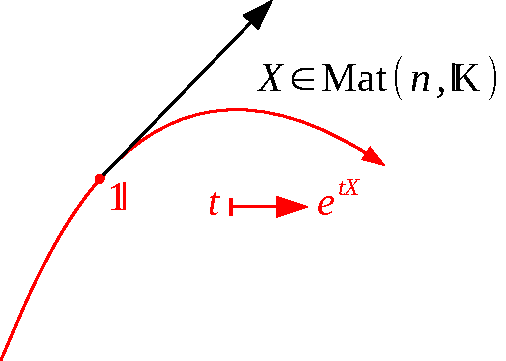
\includegraphics[width=1\linewidth]{images/derivata-exp.pdf}
	\caption{Representation of the exponential at zero as a curve with $X$ as tangent vector.}
	\labfig{derivata-exp}
\end{marginfigure}
In a sense we have this matrix $X$ which we can see as a vector in the linear space of matrices; we generate a curve which at time zero is at the identity and whose tangent vector in zero is $X$, as in \reffig{derivata-exp}.
\section{Computing the exponential}
Let us look at some special cases:

\textbf{\underline{Hp1:}} $X$ is \textbf{diagonalizable}\marginnote{This includes many interesting cases: self-adjoint, anti-self-adjoint, unitary.}. Then $\exists\;D=\mqty(\dmat{\lambda_1,\ddots,\lambda_n})$ and a similarity transformation (so an invertible matrix) $S\in\textrm{GL}(n,\mathbb{K})$ such that:\marginnote{$\underset{\cdot}{=}$ means "equivalently to"}
\[
X\underset{\cdot}{=}SDS^{-1}=S\;\mqty(\dmat{\lambda_1,\ddots,\lambda_n})\;S^{-1}
\]
Now we want to define the exponential of $X$, but we know that the exponential is well-behaved with respect to similarity transformations, so the exponential will be:
\[
e^X=e^{SDS^{-1}}=Se^DS^{-1}=S\;\mqty(\dmat{{\color{red}e^{\lambda_1}},{\color{red}\ddots},{\color{red}e^{\lambda_n}}})\;S^{-1}
\]
So if we want to exponentiate a matrix $X$ which is diagonalizable, then we diagonalize it, we exponentiate the eigenvalues and then we do the conjugation with $S$ in order to go back.
\begin{equation}\labeq{exp-oper}
{\color{red}\star \quad \Big|\Big| \qquad e^X=S\;\mqty(\dmat{e^{\lambda_1},\ddots,e^{\lambda_n}})\;S^{-1}}
\end{equation}
This is the formula which works for unbounded operators in Hilbert spaces. We know that for unbounded operators, as the Hamiltonian of an atomic or molecular system, we cannot use the exponential series, since the norm is not finite; but we can still use the formula (\ref{eq:exp-oper}).

But not every matrix is diagonalizable, what can we do? Consider the opposite case:\marginnote{In a sense there two big classes of matrices: those who are diagonalizable and those who are not (nihilpotent).}

\underline{\textbf{Hp2}:} $X$ is \textbf{nihilpotent} (\href{https://it.wikipedia.org/wiki/Nilpotente}{\textit{nilpotente}})\index{nihilpotent}, i.e. $\exists\;k:\ X^k=0$, but then, if this happens, the exponential series is finite, i.e. is a polynomial.

So how do we deal with the general case? There is a fact from linear algebra, which usually is not covered in the undergraduate courses.\marginnote[-15mm]{Questo fatto è stato usato nel corso di meccanica quantistica nella \textit{Trattazione Formale della Teoria delle Perturbazioni al Primo Ordine} [vedi Cap. 12 del Picasso \cite{picasso2015lezioni}], quando, supposto che l'Hamiltoniana $H$ di un sistema si possa scrivere nella forma
\[
H=H_0+H'
\]
dove $H_0$ è risolubile esattamente (cioè se ne conosco autovalori ed autovettori), avevamo posto
\[
H'=H'_0+H''
\]
dove $H_0'$ ha diversi da zero solo gli elementi di matrice fra autovettori di $H_0$ con la stessa energia, e $H''$ ha diversi da zero solo gli elementi di matrice fra autovettori di $H_0$ con energie diverse: $H_0'$ ha quindi, in qualunque rappresentazione in cui $H_0$ è diagonale, una struttura a blocchi. La decomposizione di $H'$ scritta sopra è unica e si ha
\[
\comm{H_0}{H_0'}=0
\]
Infatti, se  $\pazocal{P}_n$ è il proiettore sull'autospazio di $H_0$ corrispondente all'autovalore $E_n^0$, si ha $\left(\sum_n\pazocal{P}_n=\mathbb{1}\right)$:
\[
\begin{split}
    H'&\equiv \sum_{nm}\pazocal{P}_nH'\pazocal{P}_m=\\
    &=\sum_n\pazocal{P}_nH'\pazocal{P}_n+\sum_{n\neq m}\pazocal{P}_nH'\pazocal{P}_m\overset{\textrm{def}}{=}\\
    &\overset{\textrm{def}}{=}H_0'+H''
\end{split}
\]}

\underline{General case:} Every matrix $X\in\textrm{Mat}(n,\mathbb{C})$ can be written as
\begin{equation}\labeq{dec-mat}
X=A+N \qquad \begin{cases}
A \quad &\textrm{is diagonalizable}\\
N \quad &\textrm{is nihilpotent}
\end{cases}
\quad \textrm{and} \ {\color{red}\comm{A}{N}=0}
\end{equation}
Since they commute, hence $e^X=e^{A+N}\underset{\textrm{{\fontencoding{U}\fontfamily{futs}\selectfont\char 66\relax}}}{\overset{(\ref{eq:dec-mat})}{=}}\underset{\mathclap{\tikz \node {$\uparrow$} node [below=1ex] {\footnotesize compute by diagonalization };}}{e^A}\overset{\mathclap{\tikz \node {$\downarrow$} node [above=1.25ex] {\footnotesize compute by finite sums};}}{e^N}$. Of course this is nice if the index of nihilpotency\index{Index of nihilpotency} $k$ is small.
\begin{exercise}
Consider the simplest non-trivial case: $\textrm{Mat}(2,\mathbb{C})$ and consider the following two cases, one anti-symmetric and the other symmetric:
\[
X=\begin{pmatrix}
0 &-a\\
a &0
\end{pmatrix}
\qquad Y=\begin{pmatrix}
0 &b\\
b &0
\end{pmatrix}
\]
Compute $e^{tX}$ and $e^{tY}$.
\end{exercise}
%1:32:00
\section{Matrix logarithm}
\marginnote{From \cite{Presilla2014}: \textbf{Definizione (logaritmo).}\index{Logarithm definition} Sia $z\in\mathbb{C}$ con $z\neq 0$, si definisce logaritmo di $z$ ogni numero complesso
\[
\log z = \ln\abs{z}+i\arg z=\ln\abs{z}+i\left(\textrm{Arg}z+2\pi n\right)
\]
con $n\in\mathbb{Z}$ e dove $\ln(\cdot)$ indica l'usuale logaritmo naturale reale.}
\subsection{Facts from complex analysis}
We have been told at elementary school that the logarithm is not always well-defined: if we have zero or a negative number it is not well defined.
If we go to the complex plane, we know there are some forbidden points, like zero, while the logarithm of negative points makes a little sense, in the sense that it is not unique valued. 
\begin{marginfigure}
    \centering
    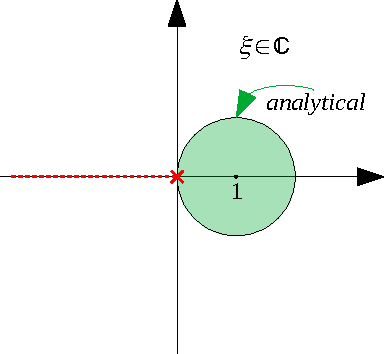
\includegraphics[width=0.7\textwidth]{images/analytical.pdf}
    \caption{Representation of the logarithm in the complex plane.}
    \labfig{analytical}
\end{marginfigure}
On the other hand, if we are around one, then things go much better. In fact, the power series (i.e. the Taylor expansion around $z=1$)
\[
\log(z)=\sum_{m=1}^{+\infty}\frac{(-1)^{m+1}}{m}(z-1)^m \qquad \Big|\Big| \quad \star
\]
is \textbf{absolutely convergent} $\forall z:{\color{red}|z-1|<1}$. Moreover, if we are inside this disk we have a return ticket: for all $z\in B_1(1_{\mathbb{C}})$
\[
e^{\log z}=z
\]
Now it comes the nasty point\marginnote{To put it smartly, "The father of the son of Zebedee, is Zebedee; but it does not mean that the son of the father of Zebedee is Zebedee", because it could be Zebedee or his brother. In a sense, it is a lack of injectivity. 

Here the son of the father of Zebedee is Zebedee, because the other brother is not so close to $0$}, things go well if we are very close to one (in one side, zero on the other). In general, the logarithm of the exponential is not derivable: $\log(e^u)\neq u$, but it is $u$ if we are very close to $0$. For all $u$ such that {\color{red}\framebox{$|u|<\log(2)$}}, we have that $|e^u-1|<1$ and it holds
\[
\log(e^u)=u
\]
If the reader do not know the details of what written above, just take it as true facts. Now we use them to define:
\begin{definition}[Matrix logarithm]\index{Matrix logarithm}\labdef{matrix-log}
For $A\in\text{Mat}(n,\mathbb{K})$ we define:
\begin{equation}\labeq{mat-log}
\log(A)=\sum_{m=1}^{+\infty}\frac{(-1)^{m+1}}{m}(A-\mathbb{1})^m
\end{equation}
\textbf{whenever the series converges.}
\end{definition}
Now we have to work a little bit to say when the series converges.
\begin{theorem}
\labthm{logA}
Defining the logarithm as the series (\ref{eq:mat-log}), therefore
\renewcommand{\labelenumi}{\Alph{enumi})}
\begin{enumerate}
    \item The series (\ref{eq:mat-log}) is \textbf{norm convergent} $\forall\; A\in\text{Mat}(n,\mathbb{K}): {\color{red}\lVert A-\mathbb{1}\rVert<1}$ and the map $A\mapsto\log(A)$ is \textbf{continuous} on $\mathbb{B}_1(\mathbb{1})$\marginnote{The notation on how to indicate the "ball" is not constant.};
    \item $\forall\;A\in\mathbb{B}_1(\mathbb{1})$ one has 
    \[
    e^{\log(A)}=A
    \]
    \item $\forall\;X\in\text{Mat}(n,\mathbb{K})$ with ${\color{red}\lVert X\rVert<\log(2)}$ then $\lVert e^X-\mathbb{1}\rVert<1$ and 
    \[
    \log(e^X)=X
    \]
\end{enumerate}
\end{theorem}
\begin{proof}
We will give just sketch of the proof, the details are left as an exercise
\renewcommand{\labelenumi}{\Alph{enumi})}
\renewcommand{\labelenumii}{\Alph{enumi}\arabic{enumii})}
\begin{enumerate}
    \item The proof is similar to what we did for the exponential $e^A$ in \refthm{expA}. We define the truncated sums
    \[
    S_N(A):=\sum_{m=1}^N\frac{(-1)^{m+1}}{m}(A-\mathbb{1})^m
    \]
    and we prove that $\{S_N(A)\}_{N\in\mathbb{N}}$ is a \textbf{Cauchy sequence} and then proceed as we did for the exponential.
    \item Suppose $\lVert A-\mathbb{1}\rVert<1$, then we have two cases:
    \begin{enumerate}
        \item Hp: $A$ is \textbf{diagonalizable} and we \textit{go back to numbers}.\marginnote{This is not always true, but it simplifies a lot the proof; then we will use it for the general case. Diagonalizable matrices are very close to numbers, up to the fact that they do not commute with each other.}
\begin{equation}\labeq{mat-log-diag}
\exists\  S\in\text{GL}(n,\mathbb{C}):(A-\mathbb{1})^m=S\begin{pmatrix}
(\lambda_1-1)^m & & 0\\
& \ddots & \\
0 & & (\lambda_n-1)^m
\end{pmatrix}
S^{-1}
\end{equation}
Notice that, as $\lVert A-\mathbb{1}\rVert<1$, each eigenvalue satisfies the analogous inequality for numbers $|\lambda_j-1|<1 \forall j\in\{1,\dots,n\}$. To see that, we use the \textbf{spectral radius}\index{Spectral radius}:\marginnote{We know from other courses that each norm is an upper bound for the spectral radius, the equality holds true for self-adjointed/unitary operators.}
\[
|\lambda_j-1|\le \sup_l|\lambda_l-1|\equiv\underset{\mathclap{\tikz \node {$\uparrow$} node [below=1ex] {\footnotesize spectral radius };}}\rho(A-\mathbb{1})\le\lVert A-\mathbb{1}\rVert<1
\]
Therefore each eigenvalue on the diagonal on the r.h.s of \refeq{mat-log-diag} is close the number one, so we can apply the power series and obtain the logarithm
\[
\sum_{m=1}^{{\color{red}N}}\frac{(-1)^{m+1}}{m}(A-\mathbb{1})^m=S\begin{pmatrix}
\ddots & & 0\\
& \sum_{m=1}^{{\color{red}N}}\frac{(-1)^{m+1}}{m}(\lambda_j-1)^m & \\
0 & & \ddots
\end{pmatrix}
S^{-1}
\]
%34:00
If now we take the limit of $N\to\infty$ on both sides, we have that, since $S$ is \textbf{continuous}, the limit goes inside the matrix on the right hand side:
\[
\log(A)=S\begin{pmatrix}
\log(\lambda_1) & & 0\\
& \ddots & \\
0 & & \log(\lambda_n)
\end{pmatrix}
S^{-1}
\]
Now that we reduced to diagonal matrices it is easy:
\[
\Rightarrow\ e^{\log(A)}=e^{S\log(D)S^{-1}}\overset{\mathclap{\tikz \node {$\downarrow$} node [above=1.25ex] {\footnotesize \refprop{exp-prop}};}}{=}Se^{\log(D)}S^{-1}\underset{\mathclap{\tikz \node {$\uparrow$} node [below=1ex] {\footnotesize Facts from complex analysis };}}{=}SDS^{-1}=A
\]
\item General case: $A$ is \textbf{non-diagonalizable}. We know from linear algebra that each $A\in\text{Mat}(n,\mathbb{C})$ can be approximated by a sequence $\{A_m\}_{m\in\mathbb{N}}$ of \textbf{diagonalizable matrices} so that $A_m$ converges in norm:
\[
A_m\xrightarrow[m\to\infty]{\lVert\dots\rVert}A
\]
    \end{enumerate}
    \item The proof is similar to B) [exercise].
\end{enumerate}
\end{proof}
\begin{starredExercise}
Prove the previous claim (B2) and complete the proof of (B).
\end{starredExercise}
What we found for numbers is that:
\[
\log(1+\varepsilon)\underset{{\varepsilon\sim0}}{\sim}\varepsilon
\]
Which can also be rewritten as:
\[
\exists\; c:\lVert\log(1+\varepsilon)-\varepsilon\rVert\le c\varepsilon^2 \quad \forall\varepsilon
\]
We will be using the second one, because is the one that generalises to matrices.
\begin{proposition}[Linear approximation of $\log(B)$]\index{Linear approximation of $\log(B)$}
$\exists\; c>0:\forall\; B\in\text{Mat}(n,\mathbb{C})$ with {\color{red}$\lVert B\rVert<\frac{1}{2}=:\varepsilon_0$} one has that:
\[
\lVert\log(\mathbb{1}+B)-B\rVert\le c\lVert B\rVert^2
\]
\end{proposition}
\begin{proof}
Using the Taylor series of the logarithm expansion
\WithArrowsOptions{displaystyle}
\begin{align*}
\begin{WithArrows}
\lVert\log\underbrace{(\mathbb{1}+B)}_{A}-B\rVert&=\lVert\sum_{m=1}^{+\infty}\frac{(-1)^{m+1}}{m}B^m-B\rVert\\
&=\lVert\sum_{{\color{red}m=2}}^{+\infty}\frac{(-1)^{m+1}}{m}B^m\rVert=\\
&=\lVert{\color{red}B^2}\sum_{m=2}^{+\infty}\frac{(-1)^{m+1}}{m}B^{m-{\color{red}2}}\rVert\le\Arrow{Trinagular inequality}\\
&\le\lVert B\rVert^2\sum_{m=2}^{+\infty}\frac{1}{m}\lVert B^{m-2}\rVert\le\Arrow{$\norm{B}< 1/2$}\\
&\le\lVert B\rVert^2\underbrace{\sum_{m=2}^{+\infty}\frac{1}{m}\left(\frac{1}{2}\right)^{m-2}}_{=:c}\Arrow{The series is convergent\\(because of 1/2)}\\
&=c\lVert B\rVert^2
\end{WithArrows}
\end{align*}
\end{proof}
\section{Further properties of the exponential}
\subsection{Lie product formula}
\begin{theorem}[Lie product formula]\index{Lie product formula}\labthm{Lie-prod-form}
$\forall\; X,Y\in\text{End}(\mathbb{C}^n)\cong\text{Mat}(n,\mathbb{C})$ one has the following:\marginnote{Immagine that in front of $X+Y$ there is a pseudotime, which has the value $1$. Now suppose we take a small time $\frac{1}{m}$. Taking the limit, we can factorize the exponential of the sum, at the price of having infinitely many factors.}
\[
e^{X+Y}=\lim_{m\to\infty}\left(e^{\frac{1}{m}X}e^{\frac{1}{m}Y}\right)^m \quad \Big|\Big| \quad \text{Lie product formula}
\]
\end{theorem}
We will use the approach of Hall \cite{Hall2015}, even if it is not the standard one, nevertheless it is based on the fact that we already know the logarithm.
\begin{proof}
Consider the power series for $m\gg1$:
\[
\begin{cases}
e^{\frac{1}{m}X}=\mathbb{1}+\frac{1}{m}X+\frac{1}{2m^2}X^2+\dots\\
e^{\frac{1}{m}Y}=\mathbb{1}+\frac{1}{m}Y+\frac{1}{2m^2}Y^2+\dots
\end{cases}
\]
We multiply them and reorganize the terms according to powers of $\frac{1}{m}$\marginnote{Consider $m$ as large, since in the end we want to take the limit}
\[
\Rightarrow\quad  e^{\frac{1}{m}X}e^{\frac{1}{m}Y}=\mathbb{1}+\frac{1}{m}X+\frac{1}{m}Y+\mathcal{O}(1/m^2)\;\xrightarrow[m\to\infty]{}\;\mathbb{1}
\]
Therefore, for $m$ sufficiently large, $\lVert e^{\frac{1}{m}X}e^{\frac{1}{m}Y}-\mathbb{1}\rVert<1$ and:
\WithArrowsOptions{displaystyle}
\[
\begin{WithArrows}
\log\left(e^{\frac{1}{m}X}e^{\frac{1}{m}Y}\right)&=\textrm{log}\Big(\mathbb{1}+\overbrace{\frac{1}{m}X+\frac{1}{m}Y+\mathcal{O}(1/m^2)}^{B}\Big)=\\
&=\frac{1}{m}X+\frac{1}{m}Y+\mathcal{O}(1/m^2)+\mathcal{O}\left(\lVert B\rVert^2\right)=\Arrow{$\norm{B}^2$ is of the order of $1/m^2$}\\
&=\frac{1}{m}X+\frac{1}{m}Y+\mathcal{O}\left(\frac{1}{m}\right)^2
\end{WithArrows}
\]
Now we exponentiate both sides and we take the limit of $m\to\infty$ (as exercise check that we are in the good region to do that):
\[
{\color{red}\lim_{m\to\infty}}\left(e^{\frac{1}{m}X}e^{\frac{1}{m}Y}\right)^{\color{red}m}={\color{red}\lim_{m\to\infty}}\left[\exp\left(\frac{1}{m}X+\frac{1}{m}Y+\mathcal{O}(1/m^2)\right)\right]^{\color{red}m}={\color{red}\lim_{m\to\infty}}e^{X+Y+\mathcal{O}(1/{\color{red}m})}\underset{\mathclap{\tikz \node {$\uparrow$} node [below=1ex] {\footnotesize $A\mapsto e^A$ is \textbf{continuous} };}}=e^{X+Y}
\]
\end{proof}
\begin{kaobox}[frametitle=Generalization: Lie-Trotter product formula] The generalization of the previous theorem is the \textbf{Lie-Trotter product formula}, which generalizes the idea to \underline{\textbf{unbounded}} self-adjoint operators in Hilbert spaces. For example, let's take the Hamiltonian of an atomic system:\marginnote{$\Delta$ is the Laplacian

The \textbf{Hartree atomic units} are a system of natural units of measurement which is especially convenient for atomic physics and computational chemistry calculations. They are named after the physicist Douglas Hartree. In this system the numerical values of the following four fundamental physical constants are all unity by definition:
\begin{itemize}
    \item Reduced Planck constant: $\hbar = 1$, also known as the \textbf{atomic unit of action}
    \item Elementary charge: $e = 1$, also known as the \textbf{atomic unit of charge}
    \item Bohr radius: $a_0 = 1$, also known as the \textbf{atomic unit of length}
    \item Electron mass: $m_\text{e} = 1$, also known as the \textbf{atomic unit of mass}
\end{itemize}
In Hartree atomic units, the speed of light is approximately 137.036 atomic units of velocity. Atomic units are often abbreviated "a.u." or "au", not to be confused with the same abbreviation used also for astronomical units, arbitrary units, and absorbance units in other contexts.}
\[
H=\underset{\mathclap{\tikz \node {$\uparrow$} node [below=1ex] {\footnotesize Kinetic energy };}}{-\Delta}+V \quad \textrm{(in Hartree units)}
\]
To keep it simple, let us specialize to one electron. The time evolution of the system is governed by the unitary group:
\[
U(t)=e^{-itH}=e^{-it(-\Delta+V)}={\color{red}\lim_{m\to\infty}}\left(e^{-i\frac{t}{m}(-\Delta)}e^{-i\frac{t}{m}(V)}\right)^m
\]
\end{kaobox}
\begin{figure}[h!]
    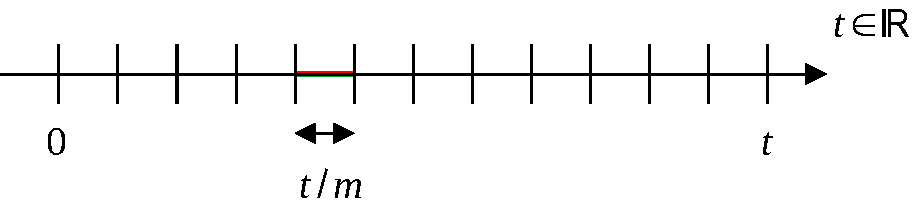
\includegraphics[width=1\textwidth]{images/lie.-trotter-pr.pdf}
    \caption*{}
\end{figure}
The limit is exact, but of course in the implementation one does finitely many steps at the price of an error. In a sense, if we want to go from $0$ to $t$, we can evolve with the full Schr\"odinger operator from $0$ to $t$, but this is difficult: in general it is not easy to diagonalize the Hamiltonian (even if Von-Neumann theorem tells us that we can always spectralize it). However, it is very easy to diagonalize the kinetic energy alone (by Fourier transformation) or to diagonalize the potential energy, which is already diagonal its position representation. And so the trick is exactly like that:
\begin{itemize}
    \item We divide our time interval in small portions, such that each one has size $\frac{t}{m}$
    \item For each of this, first we do a little bit of evolution with the kinetic energy and than a little bit with the potential
\end{itemize}
This is useful for numeric computational physics in atomic/molecular dynamics and it justifies \textbf{Feynman path integral}\index{Feynman path integral} in QM (in QFT is much more difficult, and actually there is still no satisfactory justification).
\subsection{The magic formula}
\begin{theorem}\index{Magic Formula}\labthm{MagicFormula}\marginnote{In a sense the trace and the determinant are related to each other: the trace is the tangent map of the determinant, if we forget the geometric interpretation for a moment.}
$\forall X\in\text{Mat}(n,\mathbb{K})$ we have that:
\[
{\color{red}\det(e^X)=e^{\tr(X)} \qquad \Big|\Big| \quad \star\star}
\]
\end{theorem}
\begin{proof}
We can distinguish two cases.
\begin{itemize}
    \item \underline{Case I}: $X$ is \textbf{diagonalizable}: 
\[
\exists\; S\in\text{GL}(n,\mathbb{K}): X=S\begin{pmatrix}
\lambda_1 & & 0\\
& \ddots & \\
0 & & \lambda_n
\end{pmatrix}
S^{-1}
\]
As we checked the exponential works well under conjugation
\[
e^X=S\begin{pmatrix}
e^{\lambda_1} & & 0\\
& \ddots & \\
0 & & e^{\lambda_n}
\end{pmatrix}
S^{-1}
\]
Then we can compute
\WithArrowsOptions{displaystyle}
\[
\begin{WithArrows}
\text{det}(e^X)&=\text{det}\left(Se^DS^{-1}\right)=\Arrow{Binet formula}\\
&=\cancel{\det S}\;\det(e^D)\;\cancel{\left(\det S \right)^{-1}}=\\
&=\text{det }(e^D)=\\
&=e^{\lambda_1}\dots e^{\lambda_n}=\\
&=e^{\lambda_1+\dots+\lambda_n}=\\
&=e^{\text{tr}(X)}
\end{WithArrows}
\]
\item \underline{Case II}: \marginnote{The other strategy is to write $X$ as the sum of a diagonalizable part and a nihilpotent part and work with that}$X$ is \textbf{not diagonalizable.}

$X$ can be approximated by a sequence $\{X_m\}_{m\in\mathbb{N}}$ of \textbf{diagonalizable matrices} such that $X_m\xrightarrow[m\to\infty]{}X$. Taking into account that \textbf{determinant, trace and exponential are continuous}\sidenote{some of them are even smooth}:
\WithArrowsOptions{displaystyle}
\[
\begin{WithArrows}
\det(e^X)
&=\det(e^{{\color{red}\lim_{m\to\infty}}X_m})=\\
&={\color{red}\lim_{m\to\infty}}\text{det }e^{X_m}=\Arrow{Case I}\\
&={\color{red}\lim_{m\to\infty}}e^{\text{tr}(X_m)}=\Arrow{By continuity}\\
&=e^{\tr({\color{red}\lim_{m\to\infty}}X_m)}=\\
&=e^{\text{tr}X}
\end{WithArrows}
\]
\end{itemize}
\end{proof}
\subsection{One-parameter subgroups}\marginnote{This is also something relevant for QM, even if here we define them in a finite dimensional setting.

$t$ should be interpreted as a pseudo-time}
\begin{definition}[One-parameter subgroup]\index{One-parameter subgroup}
Let $G$ be a Lie group\footnote{A general one, not necessarily a matrix Lie group}. A \textbf{one-parameter subgroup} of $G$ is a map:
\begin{align*}
A(\cdot):\mathbb{R}&\xrightarrow[]{C^0, \textrm{ hom}}G\\
t&\longmapsto A(t)
\end{align*}
which is a \textbf{continuous homomorphism of groups.} Namely:
\renewcommand{\labelenumi}{\Roman{enumi})}
\begin{enumerate}
    \item $A(\cdot)$ is continuous (= norm continuous)
    \item $A(t+s)=A(t)A(s)$
    \item $A(0)=\mathbb{1}$\marginnote{The third property is a bit redundant, since it is implied by the second.}
\end{enumerate}
\end{definition}
\paragraph{\underline{Analogy:}} In QM, $U(t)=e^{-itH}$. It can be checked that  $U(0)=\mathbb{1}$ and $U(t+s)=U(t)U(s)$. This is \textbf{strongly continuous} in the sense that if it is applied to a vector and take the limit $\varepsilon\to 0$:\marginnote{Be careful that, despite the terminology, strongly continuous is weaker than normal continuous}
\[
\lim_{\varepsilon\to 0}U(t+\varepsilon)\psi=U(t)\psi \quad \forall\psi\in\mathcal{H}
\]
So, in this infinitely dimensional case, it is \underline{\textbf{not}} true that:
\[
{\color{red}\lim_{\varepsilon\to 0}}\;\lVert U(t+\varepsilon)-U(t)\rVert_{B(H)}=0
\]
unless the Hamiltonian operator is a bounded operator $H\in B(\mathcal{H})$.
\begin{kaobox}[frametitle=Reminder]\marginnote{We ordered them from the strongest one to the weakest one}
Norm convergence > Strong convergence > Weak convergence
\end{kaobox}
In Quantum Mechanics\index{Quantum Mechanics} we have one-parameter subgroups with two differences with respect to our definition: norm continuous should be replaced by strong continuous and $G$ is equal to the group of unitaries of the Hilbert space $G=\pazocal{U}(\mathcal{H})$, which is not a Lie group in our sense, as $\dim\pazocal{U}(\mathcal{H})=+\infty$ unless $\dim\mathcal{H}<+\infty$. In toy-model, with $\dim\mathcal{H}=N$, then $G=\pazocal{U}(\mathbb{C}^N)\equiv\textrm{U}(N)$, so we are back to our Definition.
\begin{theorem}\labthm{one-par-sub}
If $A$ is a one-parameter subgroup of GL($n,\mathbb{K}$) then there exists a \textbf{unique} matrix $X\in\text{Mat}(n,\mathbb{C})$ such that 
\[
A(t)=e^{tX}
\]
\end{theorem}
To prove this theorem, we need a lemma:\marginnote[-50mm]{We enphatize on \textit{local}, because an operator can have many square roots (while a positive real number has just one square root). This is also the base of Dirac's ideas of finding a non-trivial square root of the wave operator, now called the \href{https://en.wikipedia.org/wiki/Dirac_operator}{Dirac operator}:

In mathematics and quantum mechanics, a \textbf{Dirac operator}\index{Dirac operator} is a differential operator that is a formal square root, or half-iterate, of a second-order operator such as a Laplacian. The original case which concerned Paul Dirac was to factorise formally an operator for Minkowski space, to get a form of quantum theory compatible with special relativity; to get the relevant Laplacian as a product of first-order operators he introduced spinors. It was first published in 1928.

\textbf{Formal definition}: In general, let $D$ be a first-order differential operator acting on a vector bundle $V$ over a Riemannian manifold $\mathbf{M}$. If 
\[
D^2=\Delta
\]
where $\Delta$ is the Laplacian of $V$, then $D$ is called a \textbf{Dirac operator}.

In high-energy physics, this requirement is often relaxed: only the second-order part of $D^2$ must equal the Laplacian.}
\begin{lemma}[Local square root]\index{Local square root}\lablemma{loc-square-root}
Fix $\varepsilon>0$ with $\varepsilon<\log(2)$. Consider now $\mathbb{B}_{\varepsilon/2}(0)\subseteq\text{Mat}(n,\mathbb{C})$ and define the neighborhood of the identity as
\[
{\color{black}U_{\varepsilon/2}=\exp[\mathbb{B}_{\varepsilon/2}(0)]\subseteq\text{GL}(n,\mathbb{C})}
\]
that is a subset of the general linear group, since the exponential is always invertible. Then every {\color{black}$B\in U_{\varepsilon/2}$} has a \textbf{\underline{unique} square root in} $U_{\varepsilon/2}$, explicitly given by {\color{black}$C:=e^{\frac{1}{2}\log(B)}$}.
\end{lemma}
The proof of this lemma can be found in Chapter 2 of Hall \cite{Hall2015}, what is more useful is instead a visualization of this lemma.
\begin{figure}[h!]
    \centering
    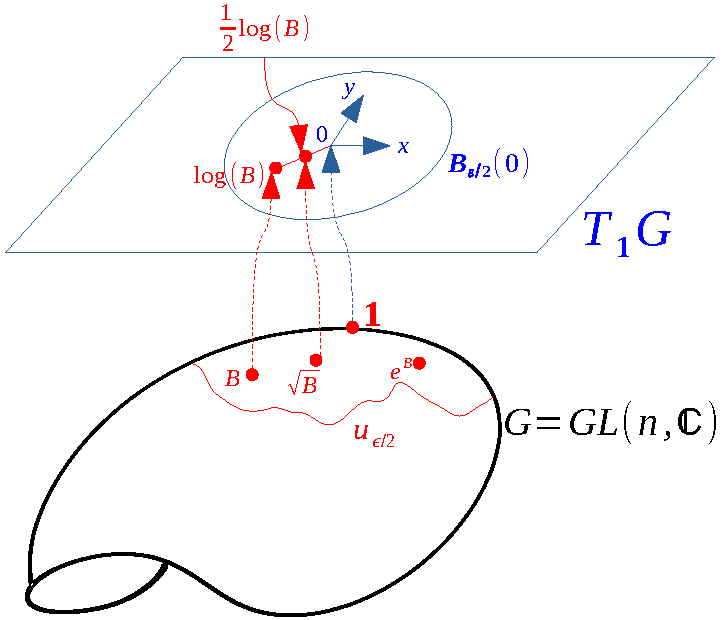
\includegraphics{images/square_root_vis.pdf}
    \caption{Visualization of the square root lemma}
    \labfig{square_root_vis}
\end{figure}
We have our group $G$ which is exactly GL$(n,\mathbb{C})$ and someone might complain since we previously stated that the general linear group is flat, in contrast to the unitary group or the orthogonal group. This is true but sometimes it is convenient to think of it as a manifold like it happens in relativity for the Minkowski space (to distinguish between space-time points and tetra-velocities, which are tangent vectors to the Minkowski space). Now we have a privileged point in the group, the identity $\mathbb{1}$, and the tangent space to $\mathbb{1}$, visualized above the manifold. There is a privileged point here too, the point 0. Now take a small neighbourhood of 0 in the tangent space upstairs, i.e. $\mathbb{B}_{\varepsilon/2}(0)$, we have some tangent vectors $x$ and $y$: from the geometric viewpoint they are tangent vectors to the group in the identity, from the practical viewpoint they are matrices. Now we can take the images of all the vectors in the ball: this will define a small set around the identity downstairs, defined as $U_{\varepsilon/2}$. Take now $B$ sufficiently close to $\mathbb{1}$, i.e. in the neighbourhood downstairs, then upstairs there is some pre-image of $B$ which is $\log B$. If it happens that $\log B$ is inside the ball, the whole segment between 0 and $\log B$ will be inside the ball: in particular, the midpoint, which is $\frac{1}{2}\log B$ will be inside the blue ball. But the blue ball and the red ball are exactly the regions in which $\log e^u=u$ and $e^{\log u}=u$ so we can easily play with them and we can go back: this will be the unique local square root of $B$, $\sqrt{B}$. 
Now we can prove the \refthm{one-par-sub}:
\begin{proof}
\circled{1} \textbf{Uniqueness}: if $A(t)=e^{tX} \quad \forall t\in\mathbb{R}$, since $e^{tX}$ is the exponential of a matrix, it is smooth in the parameter $t$ (beacuse defined by a convergent power series), so it makes sense if we derive it:
\[
\dv{}{t}e^{tX}\Bigr|_{\substack{t=0}}=Xe^{tX}\Bigr|_{\substack{t=0}}=X\quad \Rightarrow\ {\color{red}X=\dv{}{t}A(t)\Bigr|_{\substack{t=0}}}
\]
\circled{2} \textbf{Existence}: as the map $t\mapsto A(t)$ is continuous and $A(0)=\mathbb{1}$, then if time is sufficiently short, we are sufficiently close to the identity
\[
\exists\; t_0:A(t)\in U_{\varepsilon/2}\quad\forall\; t\in(-t_0,+t_0)
\]
We now define:
\[
{\color{red}X:=\frac{1}{t_0}\log(A(t_0))\qquad \Big|\Big|\quad \star}
\]
By construction, $t_0X\in\mathbb{B}_{\varepsilon/2}(0)$ and, for this particular time, it is true that $e^{t_0X}=A(t_0)$.
\begin{figure}[H]
    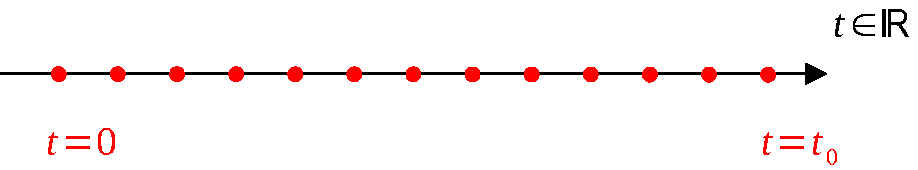
\includegraphics[width=1\textwidth]{images/ex-th-one-par-sub.pdf}
    \caption*{}
\end{figure}
We now  know that the following equality
\begin{equation}\labeq{ex-th-one-par-sub}
e^{tX}=A(t)
\end{equation}
holds true in two special points: $t=0$ and $t=t_0$. By iteration, the \refeq{ex-th-one-par-sub} will be true in a dense subset of the interval $(0,t_0)$: we can prove that if it is true in $t_0$ it is also true in $t_0/2, t_0/4,\dots$. Using now the square root \reflemma{loc-square-root} we know that $A(t_0)\in U_{\varepsilon/2}$ has a \textbf{unique local square root}:
\[
e^{\frac{t_0}{2}X}e^{\frac{t_0}{2}X}=e^{t_0X}=A(t_0)\underset{\mathclap{\tikz \node {$\uparrow$} node [below=1ex] {\footnotesize group property };}}=A(t_0/2)A(t_0/2)\qquad\Rightarrow\  A(t_0/2)=e^{\frac{t_0}{2}X}
\]
The equality on a dense set implies the equality everywhere for a continuous function and since both $e^{tX}$ and $A(t)$ are continuous, it follows that $A(t)=e^{tX}$ for all real numbers $t$. 
%(up to details that you may find in the book)\marginnote{We have also to enlarge from the interval $(-t_0,t_0)$ to the whole real line, but then we use again the good properties...}.
\end{proof}
\end{document}